\documentclass[12pt,]{article}
\usepackage{lmodern}
\usepackage{amssymb,amsmath}
\usepackage{ifxetex,ifluatex}
\usepackage{fixltx2e} % provides \textsubscript
\ifnum 0\ifxetex 1\fi\ifluatex 1\fi=0 % if pdftex
  \usepackage[T1]{fontenc}
  \usepackage[utf8]{inputenc}
\else % if luatex or xelatex
  \ifxetex
    \usepackage{mathspec}
  \else
    \usepackage{fontspec}
  \fi
  \defaultfontfeatures{Ligatures=TeX,Scale=MatchLowercase}
\fi
% use upquote if available, for straight quotes in verbatim environments
\IfFileExists{upquote.sty}{\usepackage{upquote}}{}
% use microtype if available
\IfFileExists{microtype.sty}{%
\usepackage{microtype}
\UseMicrotypeSet[protrusion]{basicmath} % disable protrusion for tt fonts
}{}
\usepackage[margin=1in]{geometry}
\usepackage{hyperref}
\hypersetup{unicode=true,
            pdftitle={STAT 6910: HW 5},
            pdfauthor={David Angeles},
            pdfborder={0 0 0},
            breaklinks=true}
\urlstyle{same}  % don't use monospace font for urls
\usepackage{color}
\usepackage{fancyvrb}
\newcommand{\VerbBar}{|}
\newcommand{\VERB}{\Verb[commandchars=\\\{\}]}
\DefineVerbatimEnvironment{Highlighting}{Verbatim}{commandchars=\\\{\}}
% Add ',fontsize=\small' for more characters per line
\usepackage{framed}
\definecolor{shadecolor}{RGB}{248,248,248}
\newenvironment{Shaded}{\begin{snugshade}}{\end{snugshade}}
\newcommand{\KeywordTok}[1]{\textcolor[rgb]{0.13,0.29,0.53}{\textbf{#1}}}
\newcommand{\DataTypeTok}[1]{\textcolor[rgb]{0.13,0.29,0.53}{#1}}
\newcommand{\DecValTok}[1]{\textcolor[rgb]{0.00,0.00,0.81}{#1}}
\newcommand{\BaseNTok}[1]{\textcolor[rgb]{0.00,0.00,0.81}{#1}}
\newcommand{\FloatTok}[1]{\textcolor[rgb]{0.00,0.00,0.81}{#1}}
\newcommand{\ConstantTok}[1]{\textcolor[rgb]{0.00,0.00,0.00}{#1}}
\newcommand{\CharTok}[1]{\textcolor[rgb]{0.31,0.60,0.02}{#1}}
\newcommand{\SpecialCharTok}[1]{\textcolor[rgb]{0.00,0.00,0.00}{#1}}
\newcommand{\StringTok}[1]{\textcolor[rgb]{0.31,0.60,0.02}{#1}}
\newcommand{\VerbatimStringTok}[1]{\textcolor[rgb]{0.31,0.60,0.02}{#1}}
\newcommand{\SpecialStringTok}[1]{\textcolor[rgb]{0.31,0.60,0.02}{#1}}
\newcommand{\ImportTok}[1]{#1}
\newcommand{\CommentTok}[1]{\textcolor[rgb]{0.56,0.35,0.01}{\textit{#1}}}
\newcommand{\DocumentationTok}[1]{\textcolor[rgb]{0.56,0.35,0.01}{\textbf{\textit{#1}}}}
\newcommand{\AnnotationTok}[1]{\textcolor[rgb]{0.56,0.35,0.01}{\textbf{\textit{#1}}}}
\newcommand{\CommentVarTok}[1]{\textcolor[rgb]{0.56,0.35,0.01}{\textbf{\textit{#1}}}}
\newcommand{\OtherTok}[1]{\textcolor[rgb]{0.56,0.35,0.01}{#1}}
\newcommand{\FunctionTok}[1]{\textcolor[rgb]{0.00,0.00,0.00}{#1}}
\newcommand{\VariableTok}[1]{\textcolor[rgb]{0.00,0.00,0.00}{#1}}
\newcommand{\ControlFlowTok}[1]{\textcolor[rgb]{0.13,0.29,0.53}{\textbf{#1}}}
\newcommand{\OperatorTok}[1]{\textcolor[rgb]{0.81,0.36,0.00}{\textbf{#1}}}
\newcommand{\BuiltInTok}[1]{#1}
\newcommand{\ExtensionTok}[1]{#1}
\newcommand{\PreprocessorTok}[1]{\textcolor[rgb]{0.56,0.35,0.01}{\textit{#1}}}
\newcommand{\AttributeTok}[1]{\textcolor[rgb]{0.77,0.63,0.00}{#1}}
\newcommand{\RegionMarkerTok}[1]{#1}
\newcommand{\InformationTok}[1]{\textcolor[rgb]{0.56,0.35,0.01}{\textbf{\textit{#1}}}}
\newcommand{\WarningTok}[1]{\textcolor[rgb]{0.56,0.35,0.01}{\textbf{\textit{#1}}}}
\newcommand{\AlertTok}[1]{\textcolor[rgb]{0.94,0.16,0.16}{#1}}
\newcommand{\ErrorTok}[1]{\textcolor[rgb]{0.64,0.00,0.00}{\textbf{#1}}}
\newcommand{\NormalTok}[1]{#1}
\usepackage{graphicx,grffile}
\makeatletter
\def\maxwidth{\ifdim\Gin@nat@width>\linewidth\linewidth\else\Gin@nat@width\fi}
\def\maxheight{\ifdim\Gin@nat@height>\textheight\textheight\else\Gin@nat@height\fi}
\makeatother
% Scale images if necessary, so that they will not overflow the page
% margins by default, and it is still possible to overwrite the defaults
% using explicit options in \includegraphics[width, height, ...]{}
\setkeys{Gin}{width=\maxwidth,height=\maxheight,keepaspectratio}
\IfFileExists{parskip.sty}{%
\usepackage{parskip}
}{% else
\setlength{\parindent}{0pt}
\setlength{\parskip}{6pt plus 2pt minus 1pt}
}
\setlength{\emergencystretch}{3em}  % prevent overfull lines
\providecommand{\tightlist}{%
  \setlength{\itemsep}{0pt}\setlength{\parskip}{0pt}}
\setcounter{secnumdepth}{0}
% Redefines (sub)paragraphs to behave more like sections
\ifx\paragraph\undefined\else
\let\oldparagraph\paragraph
\renewcommand{\paragraph}[1]{\oldparagraph{#1}\mbox{}}
\fi
\ifx\subparagraph\undefined\else
\let\oldsubparagraph\subparagraph
\renewcommand{\subparagraph}[1]{\oldsubparagraph{#1}\mbox{}}
\fi

%%% Use protect on footnotes to avoid problems with footnotes in titles
\let\rmarkdownfootnote\footnote%
\def\footnote{\protect\rmarkdownfootnote}

%%% Change title format to be more compact
\usepackage{titling}

% Create subtitle command for use in maketitle
\newcommand{\subtitle}[1]{
  \posttitle{
    \begin{center}\large#1\end{center}
    }
}

\setlength{\droptitle}{-2em}

  \title{STAT 6910: HW 5}
    \pretitle{\vspace{\droptitle}\centering\huge}
  \posttitle{\par}
    \author{David Angeles}
    \preauthor{\centering\large\emph}
  \postauthor{\par}
    \date{}
    \predate{}\postdate{}
  

\begin{document}
\maketitle

\begin{verbatim}
## Warning: package 'emmeans' was built under R version 3.4.4
\end{verbatim}

\begin{verbatim}
## NOTE: As of emmeans versions > 1.2.3,
##       The 'cld' function will be deprecated in favor of 'CLD'.
##       You may use 'cld' only if you have package:multcomp attached.
\end{verbatim}

\subsection{Problem 1}\label{problem-1}

Check the assumptions on the one-way analysis of variance model (3.3.1)
for the meat cooking experiment, which was introduced in Exercise 14 of
Chap.3. The data were given in Table 3.14. (the order of collection of
observations is not available).

The data displayed below is represented by the levels 1, 2, 3, 4, 5, and
6 which denote the frying fat content at 10\%, 15\%, and 20\% and the
grilling fat content at 10\%, 15\% and 20\% respectively for the
post-cooking weight data (in grams) for the meat cooking experiment.

\begin{Shaded}
\begin{Highlighting}[]
\KeywordTok{colnames}\NormalTok{(Post_grams) <-}\StringTok{ }\KeywordTok{c}\NormalTok{( }\StringTok{"Weight"}\NormalTok{, }\StringTok{"Code"}\NormalTok{)}
\NormalTok{Post_grams <-}\StringTok{ }\KeywordTok{data.frame}\NormalTok{(Post_grams)}
\NormalTok{Post_grams}\OperatorTok{$}\NormalTok{Code <-}\StringTok{ }\KeywordTok{factor}\NormalTok{(Post_grams}\OperatorTok{$}\NormalTok{Code)}
\KeywordTok{summary}\NormalTok{(Post_grams)}
\end{Highlighting}
\end{Shaded}

\begin{verbatim}
##      Weight      Code 
##  Min.   :71.00   1:5  
##  1st Qu.:80.00   2:5  
##  Median :82.00   3:5  
##  Mean   :81.67   4:5  
##  3rd Qu.:84.75   5:5  
##  Max.   :88.00   6:5
\end{verbatim}

\begin{Shaded}
\begin{Highlighting}[]
\NormalTok{Post_weight_model <-}\StringTok{ }\KeywordTok{aov}\NormalTok{(Weight }\OperatorTok{~}\StringTok{ }\NormalTok{Code , }\DataTypeTok{data =}\NormalTok{ Post_grams)}
\KeywordTok{anova}\NormalTok{(Post_weight_model)}
\end{Highlighting}
\end{Shaded}

\begin{verbatim}
## Analysis of Variance Table
## 
## Response: Weight
##           Df Sum Sq Mean Sq F value    Pr(>F)    
## Code       5 360.27  72.053  9.9156 3.075e-05 ***
## Residuals 24 174.40   7.267                      
## ---
## Signif. codes:  0 '***' 0.001 '**' 0.01 '*' 0.05 '.' 0.1 ' ' 1
\end{verbatim}

\begin{Shaded}
\begin{Highlighting}[]
\CommentTok{# Fitted Values}
\NormalTok{weights.fitted <-}\StringTok{ }\KeywordTok{fitted}\NormalTok{(Post_weight_model)}
\CommentTok{# Raw Residuals}
\NormalTok{weights.raw.resid <-}\StringTok{ }\KeywordTok{resid}\NormalTok{(Post_weight_model) }
\CommentTok{# Standardized Residuals}
\NormalTok{std.residuals <-}\StringTok{ }\KeywordTok{rstandard}\NormalTok{(Post_weight_model)}
\end{Highlighting}
\end{Shaded}

\begin{Shaded}
\begin{Highlighting}[]
\KeywordTok{par}\NormalTok{(}\DataTypeTok{mfrow =} \KeywordTok{c}\NormalTok{(}\DecValTok{2}\NormalTok{,}\DecValTok{2}\NormalTok{))}
\CommentTok{#Raw Residuals vs. Frying/ Grilling fat content }
\KeywordTok{plot}\NormalTok{(}\KeywordTok{as.numeric}\NormalTok{(Post_grams}\OperatorTok{$}\NormalTok{Code) , weights.raw.resid, }
     \DataTypeTok{main=} \StringTok{"Trtmt vs. Residuals"}\NormalTok{, }\DataTypeTok{xlab =} \StringTok{"Trtmt Levels"}\NormalTok{, }
     \DataTypeTok{ylab =} \StringTok{"Raw Residuals"}\NormalTok{, }\DataTypeTok{xaxt =} \StringTok{"n"}\NormalTok{,}
     \DataTypeTok{lwd =} \FloatTok{1.5}\NormalTok{)}
\KeywordTok{axis}\NormalTok{(}\DecValTok{1}\NormalTok{, }\DataTypeTok{at =} \DecValTok{1}\OperatorTok{:}\DecValTok{6}\NormalTok{, }\DataTypeTok{labels =} \KeywordTok{c}\NormalTok{(}\StringTok{"1"}\NormalTok{,}\StringTok{"2"}\NormalTok{,}\StringTok{"3"}\NormalTok{,}\StringTok{"4"}\NormalTok{,}\StringTok{"5"}\NormalTok{,}\StringTok{"6"}\NormalTok{))}
\KeywordTok{abline}\NormalTok{(}\DataTypeTok{h=}\DecValTok{0}\NormalTok{, }\DataTypeTok{col =} \StringTok{"red"}\NormalTok{, }\DataTypeTok{lty =} \DecValTok{2}\NormalTok{)}

\CommentTok{#Raw Residuals vs. Fitted Values}
\KeywordTok{plot}\NormalTok{(weights.fitted , weights.raw.resid, }
     \DataTypeTok{main=} \StringTok{"Fitted Values vs. Residuals"}\NormalTok{, }\DataTypeTok{xlab =} \StringTok{"Fitted Values"}\NormalTok{, }
     \DataTypeTok{ylab =} \StringTok{"Raw Residuals"}\NormalTok{,}
     \DataTypeTok{lwd =} \FloatTok{1.5}\NormalTok{)}
\KeywordTok{abline}\NormalTok{(}\DataTypeTok{h=}\DecValTok{0}\NormalTok{, }\DataTypeTok{col =} \StringTok{"red"}\NormalTok{, }\DataTypeTok{lty =} \DecValTok{2}\NormalTok{)}

\CommentTok{#Standardized Residuals vs. Fitted Values}
\KeywordTok{plot}\NormalTok{(weights.fitted , std.residuals, }
     \DataTypeTok{main=} \StringTok{"Trtmt vs. Std. Residuals"}\NormalTok{, }\DataTypeTok{xlab =} \StringTok{"Fitted Values"}\NormalTok{, }
     \DataTypeTok{ylab =} \StringTok{"Standardize Residuals"}\NormalTok{,}
     \DataTypeTok{lwd =} \FloatTok{1.5}\NormalTok{)}
\KeywordTok{abline}\NormalTok{(}\DataTypeTok{h=}\DecValTok{0}\NormalTok{, }\DataTypeTok{col =} \StringTok{"red"}\NormalTok{, }\DataTypeTok{lty =} \DecValTok{2}\NormalTok{)}

\CommentTok{#Norma Probability Plot}
\KeywordTok{qqnorm}\NormalTok{(weights.raw.resid, }\DataTypeTok{main=} \StringTok{"Normal Q-Q Plot of Raw Residuals"}\NormalTok{)}
\KeywordTok{qqline}\NormalTok{(weights.raw.resid, }\DataTypeTok{col =} \StringTok{"red"}\NormalTok{)}
\end{Highlighting}
\end{Shaded}

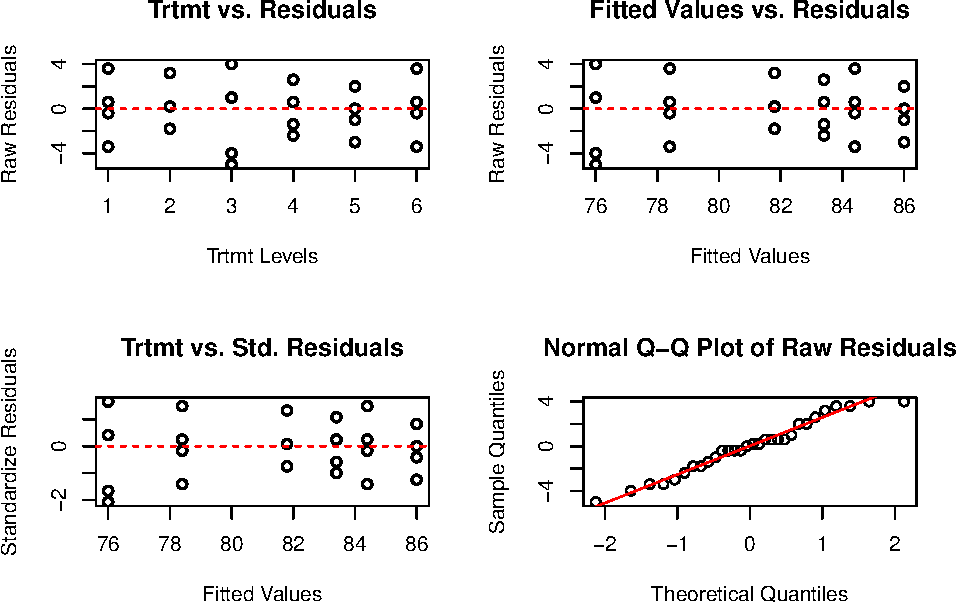
\includegraphics{Markdown_HW_5_files/figure-latex/unnamed-chunk-5-1.pdf}

Assumption (a): The error have mean 0:

Due to the formulation of the One Way ANOVA Model, the residuals always
sum up to 0. Hence, the assumption cannot be checked.

Assumption (b): The error have constant variance:

\begin{Shaded}
\begin{Highlighting}[]
\NormalTok{vars<-}\StringTok{ }\KeywordTok{tapply}\NormalTok{(Post_grams}\OperatorTok{$}\NormalTok{Weight,Post_grams}\OperatorTok{$}\NormalTok{Code, var)}
\KeywordTok{max}\NormalTok{(vars)}\OperatorTok{/}\KeywordTok{min}\NormalTok{(vars)}
\end{Highlighting}
\end{Shaded}

\begin{verbatim}
## [1] 4.868421
\end{verbatim}

Using the rule of thumb based on within group variances we can see that
\[\frac{\max_i\{S_i^2 \}}{\min_i\{S_i^2 \}} =\frac{18.5}{3.8} = 4.87.\]
However, by plotting the standardized residuals against the fitted
values and the treatment levels we saw no big difference in the pattern
of the spread within the groups. Therefore, the
\(\frac{\max_i\{S_i^2 \}}{\min_i\{S_i^2 \}}\) result can simply be due
to the fact that the sample sizes of each group is only 4. So we feel
comfortable that the equal variance assumption is approximately
satisfied.

Assumption (c): The error are normally distributed:

From the qq-plot above we see that the data is fairly straight.
Furthermore, all the standardized residuals are \(|z_i| \leq 2.074\), so
we don't have any apparent outliers. Therefore the normality assumption
is reasonable.

\begin{Shaded}
\begin{Highlighting}[]
\KeywordTok{max}\NormalTok{(}\KeywordTok{abs}\NormalTok{(std.residuals))}
\end{Highlighting}
\end{Shaded}

\begin{verbatim}
## [1] 2.073755
\end{verbatim}

Assumption (d): The errors are independent:

Since we do not have any information on how the data was collected, we
can't verify the Independence assumption.

\subsection{Problem 2}\label{problem-2}

The spaghetti sauce experiment was run to compare the thicknesses of
three particular brands of spaghetti sauce, both when stirred and
unstirred. The six treatments were:

\begin{center}
1 = store brand, unstirred 2 = store brand, stirred\\
3 = national brand, unstirred 4 = national brand, stirred \\ 
5=gourmet brand,unstirred 6=gourmet brand,stirred
\end{center}

Part of the data collected is shown in Table 5.22. There are three
observations per treatment, and the response variable is the weight (in
grams) of sauce that flowed through a colander in a given period of
time. A thicker sauce would give rise to smaller weights.

\begin{enumerate}
\def\labelenumi{(\alph{enumi})}
\tightlist
\item
  Check the assumptions on the one-way analysis of variance model
  (3.3.1).
\end{enumerate}

\begin{Shaded}
\begin{Highlighting}[]
\NormalTok{spaghetti.data =}\StringTok{ }\KeywordTok{read.table}\NormalTok{(}\StringTok{"~/Desktop/Stats 6910/HW_4_and_5/spaghetti.sauce.txt"}\NormalTok{, }\DataTypeTok{header =} \OtherTok{TRUE}\NormalTok{)}

\NormalTok{spaghetti.model =}\StringTok{ }\KeywordTok{aov}\NormalTok{(weight }\OperatorTok{~}\StringTok{ }\KeywordTok{factor}\NormalTok{(trtmt), spaghetti.data)}
\CommentTok{# Compute predicted values, residuals, standardized residuals, normal scores}
\NormalTok{spaghetti.data =}\StringTok{ }\KeywordTok{within}\NormalTok{(spaghetti.data, \{}
  \CommentTok{# Compute predicted, residual, and standardized residual values}
\NormalTok{  ypred =}\StringTok{ }\KeywordTok{fitted}\NormalTok{(spaghetti.model)}
\NormalTok{  e =}\StringTok{ }\KeywordTok{resid}\NormalTok{(spaghetti.model) }
\NormalTok{  z =}\StringTok{ }\KeywordTok{rstandard}\NormalTok{(spaghetti.model)\})}
\CommentTok{# Display first 10 lines of mung.data, 4 digits per variable}
\KeywordTok{print}\NormalTok{(}\KeywordTok{head}\NormalTok{(spaghetti.data, }\DecValTok{10}\NormalTok{), }\DataTypeTok{digits=}\DecValTok{4}\NormalTok{)}
\end{Highlighting}
\end{Shaded}

\begin{verbatim}
##    order trtmt weight brand stir       z       e ypred
## 1      1     3     14     2    1 -0.9138 -3.0000 17.00
## 2      2     2     69     1    2  1.0153  3.3333 65.67
## 3      3     4     26     2    2  0.9138  3.0000 23.00
## 4      4     3     15     2    1 -0.6092 -2.0000 17.00
## 5      5     4     20     2    2 -0.9138 -3.0000 23.00
## 6      6     5     12     3    1 -1.0153 -3.3333 15.33
## 7      7     1     55     1    1 -0.9138 -3.0000 58.00
## 8      8     6     14     3    2 -0.5077 -1.6667 15.67
## 9      9     6     16     3    2  0.1015  0.3333 15.67
## 10    10     5     16     3    1  0.2031  0.6667 15.33
\end{verbatim}

\begin{Shaded}
\begin{Highlighting}[]
\CommentTok{# Generate residual plots}

\KeywordTok{par}\NormalTok{(}\DataTypeTok{mfrow =} \KeywordTok{c}\NormalTok{(}\DecValTok{2}\NormalTok{,}\DecValTok{2}\NormalTok{))}
\KeywordTok{plot}\NormalTok{(z }\OperatorTok{~}\StringTok{ }\NormalTok{trtmt, }\DataTypeTok{data=}\NormalTok{spaghetti.data, }
      \DataTypeTok{main=} \StringTok{"Trtmt vs. Std. Residuals"}\NormalTok{,}
     \DataTypeTok{ylab=}\StringTok{"Std. Residuals"}\NormalTok{, }\DataTypeTok{las=}\DecValTok{1}\NormalTok{)}
\KeywordTok{abline}\NormalTok{(}\DataTypeTok{h=}\DecValTok{0}\NormalTok{)  }\CommentTok{# Horizontal line at zero}
\KeywordTok{plot}\NormalTok{(z }\OperatorTok{~}\StringTok{ }\NormalTok{order, }\DataTypeTok{data=}\NormalTok{spaghetti.data, }
     \DataTypeTok{main=} \StringTok{"Order vs. Std. Residuals"}\NormalTok{,}
     \DataTypeTok{ylab=}\StringTok{"Std. Residuals"}\NormalTok{, }\DataTypeTok{las=}\DecValTok{1}\NormalTok{)}
\KeywordTok{abline}\NormalTok{(}\DataTypeTok{h=}\DecValTok{0}\NormalTok{)}
\KeywordTok{plot}\NormalTok{(z }\OperatorTok{~}\StringTok{ }\NormalTok{ypred, }\DataTypeTok{data=}\NormalTok{spaghetti.data, }
      \DataTypeTok{main=} \StringTok{"Fitted Values vs. Std. Residuals"}\NormalTok{,}
     \DataTypeTok{ylab=}\StringTok{"Std. Residuals"}\NormalTok{, }\DataTypeTok{las=}\DecValTok{1}\NormalTok{)}
\KeywordTok{abline}\NormalTok{(}\DataTypeTok{h=}\DecValTok{0}\NormalTok{)}
\KeywordTok{qqnorm}\NormalTok{(spaghetti.data}\OperatorTok{$}\NormalTok{z)}
\CommentTok{# Line through 1st and 3rd quantile points}
\KeywordTok{qqline}\NormalTok{(spaghetti.data}\OperatorTok{$}\NormalTok{z) }
\end{Highlighting}
\end{Shaded}

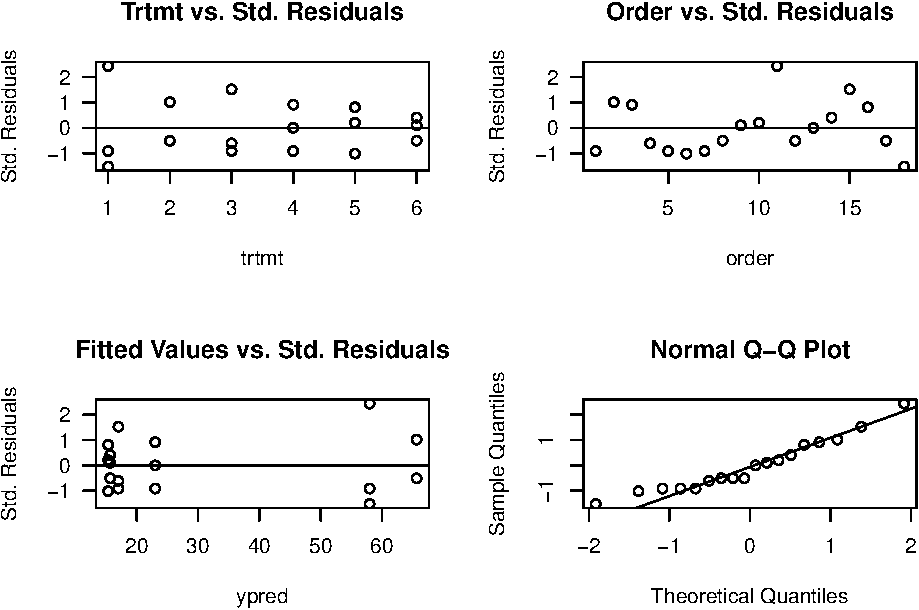
\includegraphics{Markdown_HW_5_files/figure-latex/unnamed-chunk-8-1.pdf}

Assumption (a): The error have mean 0:

Due to the formulation of the One Way ANOVA Model, the residuals always
sum up to 0. Hence, the assumption cannot be checked.

Assumption (b): The error have constant variance:

\begin{Shaded}
\begin{Highlighting}[]
\NormalTok{Y_i_var <-}\StringTok{ }\KeywordTok{tapply}\NormalTok{(spaghetti.data}\OperatorTok{$}\NormalTok{weight, spaghetti.data}\OperatorTok{$}\NormalTok{trtmt, var);}
\KeywordTok{max}\NormalTok{(Y_i_var)}\OperatorTok{/}\KeywordTok{min}\NormalTok{(Y_i_var)}
\end{Highlighting}
\end{Shaded}

\begin{verbatim}
## [1] 21
\end{verbatim}

Using the rule of thumb based on within group variances we can see that
\[\frac{\max_i\{S_i^2 \}}{\min_i\{S_i^2 \}} =\frac{49}{2.33} = 21.\]
Furthermore, by plotting the standardized residuals against the fitted
values we can see that the spread of the standardized residuals
increases as the fitted values increase. Hence, with these two results
we feel comfortable to say that the equal variance assumption is not
satisfied.

Assumption (c): The error are normally distributed:

From the qq-plot above we see that the data is fairly straight.
Furthermore, all the standardized residuals are \(|z_i| \leq 2.437\), so
we don't have any apparent outliers. Therefore, the normality assumption
is reasonable.

\begin{Shaded}
\begin{Highlighting}[]
\KeywordTok{max}\NormalTok{(}\KeywordTok{abs}\NormalTok{(spaghetti.data}\OperatorTok{$}\NormalTok{z))}
\end{Highlighting}
\end{Shaded}

\begin{verbatim}
## [1] 2.436831
\end{verbatim}

Assumption (d): The errors are independent:

From the plot of Order vs.~Residuals we can see that there isn't a
pattern as time increases. Therefore we feel comfortable that the errors
are approximately satisfies.

\begin{enumerate}
\def\labelenumi{(\alph{enumi})}
\setcounter{enumi}{1}
\tightlist
\item
  Use Satterthwaite's method to obtain simultaneous confidence intervals
  for the six preplanned contrasts
\end{enumerate}

\[\tau_1 -\tau_2, \tau_3 -\tau_4, \tau_5 -\tau_6, \tau_1 -\tau_5, \tau_1 -\tau_3, \tau_3 -\tau_5,\]

Select an overall confidence level of at least 95\%.

We will use Tukey's method of multiple comparison since we want a
simultaneous confidence intervals for the preplanned contrasts. Although
Tukey's method gives confidence intervals for all pairwise comparison,
we will only display the ones requested. Therefore,

\begin{center}
A simultaneous confidence interval for $\tau_1 -\tau_2$ is $(-34.96928,19.63595)$.\\
A simultaneous confidence interval for $\tau_3 -\tau_4$ is $(-21.516045,9.516045)$.\\
A simultaneous confidence interval for $\tau_5 -\tau_6$ is $(-11.70676,11.04009)$.\\
A simultaneous confidence interval for $\tau_1 -\tau_5$ is $(15.74657,69.58676)$.\\
A simultaneous confidence interval for $\tau_1 -\tau_3$ is $(15.92339,66.07661)$.\\
A simultaneous confidence interval for $\tau_3 -\tau_5$ is $(-13.84765,17.18098)$.
\end{center}

The work is shown in the code below.

\begin{Shaded}
\begin{Highlighting}[]
\CommentTok{# Fitted values}
\NormalTok{Y_i_hat <-}\StringTok{ }\KeywordTok{tapply}\NormalTok{(spaghetti.data}\OperatorTok{$}\NormalTok{weight, spaghetti.data}\OperatorTok{$}\NormalTok{trtmt, mean);}
\CommentTok{# Sample Variance}
\NormalTok{Y_i_var <-}\StringTok{ }\KeywordTok{tapply}\NormalTok{(spaghetti.data}\OperatorTok{$}\NormalTok{weight, spaghetti.data}\OperatorTok{$}\NormalTok{trtmt, var);}


\CommentTok{# Confidence Interval for tau_i - tau_j}
\NormalTok{CI_Satterthwaite <-}\StringTok{ }\ControlFlowTok{function}\NormalTok{(ti,tj,variance_i,variance_j,r,v)\{}
\CommentTok{# Numerator for Degree of Freedom}
\NormalTok{numerator <-}\StringTok{ }\KeywordTok{sum}\NormalTok{(variance_i}\OperatorTok{/}\NormalTok{r,variance_j}\OperatorTok{/}\NormalTok{r)}\OperatorTok{^}\DecValTok{2}
\CommentTok{# Denominator for Degree of Freedom}
\NormalTok{denominator <-}\StringTok{ }\KeywordTok{sum}\NormalTok{((variance_i}\OperatorTok{/}\NormalTok{r)}\OperatorTok{^}\DecValTok{2}\OperatorTok{/}\NormalTok{(r}\OperatorTok{-}\DecValTok{1}\NormalTok{), (variance_j}\OperatorTok{/}\NormalTok{r)}\OperatorTok{^}\DecValTok{2}\OperatorTok{/}\NormalTok{(r}\OperatorTok{-}\DecValTok{1}\NormalTok{))}
\CommentTok{#Degrees of freedom}
\NormalTok{deg.fr_taui_tauj <-}\StringTok{ }\NormalTok{numerator}\OperatorTok{/}\StringTok{ }\NormalTok{denominator}
\KeywordTok{print}\NormalTok{(deg.fr_taui_tauj)}
\CommentTok{#Standard error}
\NormalTok{SE <-}\StringTok{ }\KeywordTok{sqrt}\NormalTok{(}\KeywordTok{sum}\NormalTok{(variance_i}\OperatorTok{/}\NormalTok{r,variance_j}\OperatorTok{/}\NormalTok{r))}
\CommentTok{# w_T}
\NormalTok{w_T <-}\StringTok{ }\KeywordTok{qtukey}\NormalTok{(.}\DecValTok{95}\NormalTok{,v,deg.fr_taui_tauj)}\OperatorTok{/}\StringTok{ }\KeywordTok{sqrt}\NormalTok{(}\DecValTok{2}\NormalTok{)}
\CommentTok{# tau_i - tau_j}
\NormalTok{ti_minus_tj <-}\StringTok{ }\NormalTok{ti }\OperatorTok{-}\StringTok{ }\NormalTok{tj}
\CommentTok{#return confidence interval}
\KeywordTok{return}\NormalTok{(CI_ti_minus_tj <-}\KeywordTok{c}\NormalTok{(ti_minus_tj }\OperatorTok{-}\StringTok{ }\NormalTok{w_T }\OperatorTok{*}\StringTok{ }\NormalTok{SE,ti_minus_tj }\OperatorTok{+}\StringTok{ }\NormalTok{w_T }\OperatorTok{*}\StringTok{ }\NormalTok{SE))}
\NormalTok{\}}

\NormalTok{t_i <-}\StringTok{ }\KeywordTok{c}\NormalTok{(}\DecValTok{1}\NormalTok{,}\DecValTok{3}\NormalTok{,}\DecValTok{5}\NormalTok{,}\DecValTok{1}\NormalTok{,}\DecValTok{1}\NormalTok{,}\DecValTok{3}\NormalTok{)}
\NormalTok{t_j <-}\StringTok{ }\KeywordTok{c}\NormalTok{(}\DecValTok{2}\NormalTok{,}\DecValTok{4}\NormalTok{,}\DecValTok{6}\NormalTok{,}\DecValTok{5}\NormalTok{,}\DecValTok{3}\NormalTok{,}\DecValTok{5}\NormalTok{)}
\NormalTok{CI_ti_minus_tj <-}\StringTok{ }\OtherTok{NULL}

\ControlFlowTok{for}\NormalTok{ (i }\ControlFlowTok{in} \DecValTok{1}\OperatorTok{:}\DecValTok{6}\NormalTok{)\{}
\NormalTok{CI_ti_minus_tj<-}\KeywordTok{rbind}\NormalTok{(CI_ti_minus_tj,}
\KeywordTok{CI_Satterthwaite}\NormalTok{(Y_i_hat[t_i[i]],Y_i_hat[t_j[i]],}
\NormalTok{                 Y_i_var[t_i[i]],Y_i_var[t_j[i]],}\DecValTok{3}\NormalTok{,}\DecValTok{6}\NormalTok{)) \}}
\end{Highlighting}
\end{Shaded}

\begin{verbatim}
## [1] 2.66115
## [1] 3.547511
## [1] 2.941176
## [1] 2.73523
## [1] 3.348298
## [1] 3.582941
\end{verbatim}

\begin{Shaded}
\begin{Highlighting}[]
\KeywordTok{colnames}\NormalTok{(CI_ti_minus_tj) <-}\StringTok{ }\KeywordTok{c}\NormalTok{(}\StringTok{"Lower"}\NormalTok{,}\StringTok{"Upper"}\NormalTok{)}
\NormalTok{CI_ti_minus_tj}
\end{Highlighting}
\end{Shaded}

\begin{verbatim}
##          Lower     Upper
## [1,] -34.96928 19.635948
## [2,] -21.51604  9.516045
## [3,] -11.70676 11.040092
## [4,]  15.74657 69.586762
## [5,]  15.92339 66.076609
## [6,] -13.84765 17.180981
\end{verbatim}


\end{document}
